\subsection{Voorbeelden}

\begin{voorbeeld}
	Bespreek de functie $f$ met voorschrift $f(x)=\sqrt{10-2x}-2$.

%\begin{figure}[h]
	%\centering{}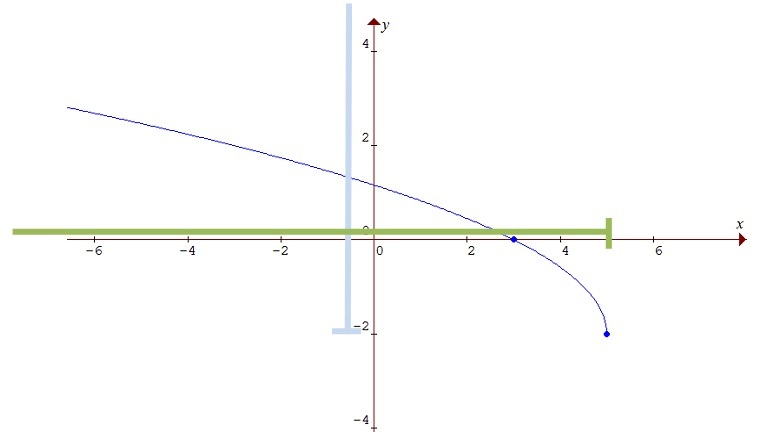
\includegraphics[height=5cm]{2_elem_rekenvaardigheden_B/inputs/reeel_vb1.jpg} 
%\end{figure}

%TODO figuur inladen 
\begin{figure}
	\centering          
	\tikzsetfigurename{Fig_module_2_1_2_reele_functies_vb1}
%TODO polynoombenadering uitrekenen > zie cursus Algebra

\begin{tikzpicture}[cap=round]

% Styles
\tikzstyle{axes}=[]
\tikzstyle help lines=[color=blue!50,very thin,dotted]


%%%%%%%%%%%%%%%%%%%%%%%%%%%%%%%%
%		GRID
%%%%%%%%%%%%%%%%%%%%%%%%%%%%%%%%

\draw[style=help lines,step=1cm] (-6.9,-3.9) grid (6.9,3.9);



%%%%%%%%%%%%%%%%%%%%%%%%%%%%%%%%
%		ASSENSTELSEL
%%%%%%%%%%%%%%%%%%%%%%%%%%%%%%%%

\draw[->] (-7,0) -- (7,0) node[right] {$x$};
\draw[->] (0,-4) -- (0,4) node[left]{$y$};

%\draw[fill,cyan](1,1)circle [radius=0.025];

%\draw[red,cap=rect, loosely dashed, ultra thick, domain=-2:2] plot (\x, {(\x*\x-1)+0.05}) node[above,yshift=-.7cm, right]{};

%%%%%%%%%%%%%%%%%%%%%%%%%%%%%%%%
%legende
%%%%%%%%%%%%%%%%%%%%%%%%%%%%%%%%
%\tkzDefPoint(0.5,3.5){A}
%\tkzDefPoint(1,3.5){B}
%\tkzLabelPoint[right,xshift=+0.1cm](B){${\color{cyan}f(x)=|x^2-1|}$}
%\tkzDrawSegment[cyan,ultra thick](A,B)

%\tkzDefPoint(0.5,3.2){C}
%\tkzDefPoint(1,3.2){D}
%\tkzLabelPoint[right,xshift=+0.1cm](D){${\color{red}e(x)=x^2-1}$}
%\tkzDrawSegment[red,cap=rect, loosely dashed, ultra thick](C,D)


%%%%%%%%%%%%%%%%%%%%%%%%%%%%%%%%
%getallen op de x-as en lijntjes
%%%%%%%%%%%%%%%%%%%%%%%%%%%%%%%%   
\foreach \x/\xtext in {-6,-5,-4,-3,-2,-1,1,2,3,4,5,6}
	\draw[xshift=\x cm] (0pt,1pt) -- (0pt,0pt) node[below,fill=white]
	{$\xtext$};,3
	
%getallen op de y-as en lijntjes  
%BEGIN LUS
\foreach \y/\ytext in {-4,-3,-2,-1,1,2,3}
	\draw[yshift=\y cm] (1pt,0pt) -- (0pt,0pt) node[left,fill=white]
	{$\ytext$}; %EINDE LUS



%%%%%%%%%%%%%%%%%%%%%%%%%%%%%%%%
%		GRAFIEKEN
%%%%%%%%%%%%%%%%%%%%%%%%%%%%%%%%
%\draw[cyan,cap=rect,thick, domain=-6:6] plot (\x, \x) node[above, right]{${\color{cyan}y=x}$};v

%\draw[cyan,cap=rect,ultra thick, domain=-6:1.75] plot (\x, {(\x-2)^(-1)}) node[above,right]{};


%\draw[cyan,cap=rect,ultra thick, domain=2.25:6] plot (\x, {(\x-2)^(-1)}) node[above,yshift=+0.5cm,left]{$\color{cyan} y=\frac{1}{x-2}$};


%\draw[cyan,cap=rect,ultra thick, domain=-7:1.9] plot (\x, {exp{\x}}) node[above, right]{${\color{cyan}y=\exp{x}}$};

%%%%%%%%%%%%%%%%%%%%%%%%%%%%%%%%
%		MARKERINGEN
%%%%%%%%%%%%%%%%%%%%%%%%%%%%%%%%
%verticale lijn
\draw[-o,line width=4,teal, cap=rect,opacity=0.3] (0,-4) -- (0,0.25) node[right] {};
\draw[line width=4,teal, cap=rect,opacity=0.3] (0,0) -- (0,4.2) node[right] {bld $f$ = $\mathbb{R}_0$};
%horizontale lijn
\draw[arrows=-o,line width=4,blue, cap=rect,opacity=0.3] (-7,0) -- (2.25,0) node[right] {};
\draw[line width=4,blue, cap=rect,opacity=0.3] (2.25,0) -- (7,0) node[below,yshift=-0.3cm] {dom$f$ = $\mathbb{R}  \setminus 2 $};
 
\end{tikzpicture}

	\caption{voorbeeld 1}
\label{fig:reele_functies_vb1}	
\end{figure}



\textbf{Domein}: de uitdrukking onder de vierkantswortel
mag niet negatief worden:


\begin{eqnarray*}
	\begin{array}{cccc}
		& 10-2x & \geqslant & 0\\
		\iff & 10 & \geqslant & 2x\\
		\iff & 5 & \geqslant & x\\
		\iff & x & \leqslant & 5
	\end{array}
\end{eqnarray*}


Besluit: voor $x$ zijn alle waarden van $-\infty$ tot
en met $5$ toegelaten. We schrijven: $\textrm{dom}\ f(x)=]-\infty,5]$ 

\textbf{Beeld}: de kleinste functiewaarde wordt
bekomen als de wortel $0$ is. Vierkantwortels geven altijd een positief
resultaat (of nul). De uitdrukking onder de wortel wordt $0$ als
$x=5$. We zien dat $f(5)=-2$. Er is geen bovengrens, dus het bereik
loopt tot $+\infty$.

Besluit: $\textrm{bld}f=[-2,+\infty[$




\textbf{Nulpunten}: voor welke waarden van $x$ wordt $f(x)=0$?


\begin{eqnarray*}
	\begin{array}{cccc}
		& \sqrt{10-2x}-2 & = & 0\\
		\iff & \sqrt{10-2x} & = & 2\\
		\iff & \left(\sqrt{10-2x}\right)^{2} & = & 2^{2}\\
		\iff & 10-2x & = & 4\\
		\iff & 6 & = & 2x\\
		\iff & x & = & 3
	\end{array}
\end{eqnarray*}


Besluit: er is slechts 1 nulwaarde, en dit is $x=3$ .




\textbf{Symmetrie}: we gaan na of het beeld van $-x$ hetzelfde
of het tegengestelde resultaat geeft als de gegeven functie. $f(-x)=\sqrt{10-2(-x)}-2=\sqrt{10+2x}-2$.
Dit is noch gelijk aan $f(x)$ noch gelijk aan $-f(x)$. Deze functie
is dus noch even, noch oneven.

\end{voorbeeld}

\begin{voorbeeld}
	Bespreek de functie met voorschrift $f(x)=\frac{1}{x-2}$.

%\begin{figure}[h]
%	\centering{}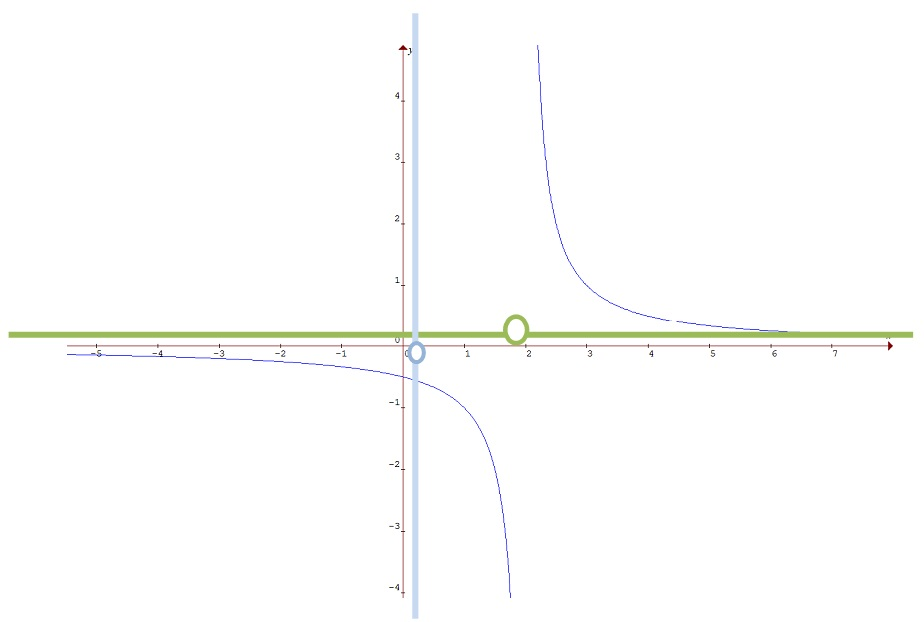
\includegraphics[height=5cm]{2_elem_rekenvaardigheden_B/inputs/reeel_vb2.jpg} 
%\end{figure}

%TODO figuur inladen

\begin{figure}
	\centering          
	
\begin{center}
\begin{tikzpicture}[scale=1,cap=round]

% Styles
\tikzstyle{axes}=[]
\tikzstyle help lines=[color=blue!50,very thin,dotted]


%%%%%%%%%%%%%%%%%%%%%%%%%%%%%%%%
%		GRID
%%%%%%%%%%%%%%%%%%%%%%%%%%%%%%%%

\draw[style=help lines,step=1cm] (-3.9,-5.9) grid (3.9,5.9);



%%%%%%%%%%%%%%%%%%%%%%%%%%%%%%%%
%		ASSENSTELSEL
%%%%%%%%%%%%%%%%%%%%%%%%%%%%%%%%

\draw[->] (-5,0) -- (5,0) node[right] {$x$};
\draw[->] (0,-7) -- (0,7) node[left]{$y$};

%\draw[fill,cyan](1,1)circle [radius=0.025];

%\draw[red,cap=rect, loosely dashed, ultra thick, domain=-2:2] plot (\x, {(\x*\x-1)+0.05}) node[above,yshift=-.7cm, right]{};

%%%%%%%%%%%%%%%%%%%%%%%%%%%%%%%%
%legende
%%%%%%%%%%%%%%%%%%%%%%%%%%%%%%%%
%\tkzDefPoint(0.5,3.5){A}
%\tkzDefPoint(1,3.5){B}
%\tkzLabelPoint[right,xshift=+0.1cm](B){${\color{cyan}f(x)=|x^2-1|}$}
%\tkzDrawSegment[cyan,ultra thick](A,B)

%\tkzDefPoint(0.5,3.2){C}
%\tkzDefPoint(1,3.2){D}
%\tkzLabelPoint[right,xshift=+0.1cm](D){${\color{red}e(x)=x^2-1}$}
%\tkzDrawSegment[red,cap=rect, loosely dashed, ultra thick](C,D)


%%%%%%%%%%%%%%%%%%%%%%%%%%%%%%%%
%getallen op de x-as en lijntjes
%%%%%%%%%%%%%%%%%%%%%%%%%%%%%%%%   
\foreach \x/\xtext in {-4,-3,-2,-1,1,2,3,4}
	\draw[xshift=\x cm] (0pt,1pt) -- (0pt,0pt) node[below,fill=white]
	{$\xtext$};,3
	
%getallen op de y-as en lijntjes  
%BEGIN LUS
\foreach \y/\ytext in {-6,-5,-4,-3,-2,-1,1,2,3,4,5,6}
	\draw[yshift=\y cm] (1pt,0pt) -- (0pt,0pt) node[left,fill=white]
	{$\ytext$}; %EINDE LUS



%%%%%%%%%%%%%%%%%%%%%%%%%%%%%%%%
%		GRAFIEKEN
%%%%%%%%%%%%%%%%%%%%%%%%%%%%%%%%
%\draw[cyan,cap=rect,thick, domain=-6:6] plot (\x, \x) node[above, right]{${\color{cyan}y=x}$};

\draw[cyan,cap=rect,ultra thick, domain=-1.2:3.5] plot (\x, {
	pow(\x,3)-3*pow(\x,2)		% <- plaats het functievoorschrift hier
}) node[above]{$f(x)=x^3-3x^2$};

\draw[opacity=0] (-1.2,-5) --(-1,-3) node[opacity=1,blue, midway,sloped]{stijgen};  
\draw[opacity=0] (0.5,-1) --(1.3,-3) node[opacity=1,blue, midway,sloped,above]{dalen};  
\draw[opacity=0] (3,1) --(3.5,5) node[opacity=1,blue, midway,sloped,above]{stijgen};  


%node[blue]{stijgen} 
%\draw[cyan,cap=rect,ultra thick, domain=2.25:6] plot (\x, {(\x-2)^(-1)}) node[above,yshift=+0.5cm,left]{$\color{cyan} y=\frac{1}{x-2}$};


%\draw[cyan,cap=rect,ultra thick, domain=-7:1.9] plot (\x, {exp{\x}}) node[above, right]{${\color{cyan}y=\exp{x}}$};

%%%%%%%%%%%%%%%%%%%%%%%%%%%%%%%%
%		MARKERINGEN
%%%%%%%%%%%%%%%%%%%%%%%%%%%%%%%%
%verticale lijn
%\draw[-o,line width=4,teal, cap=rect,opacity=0.3] (0,-4) -- (0,0.25) node[right] {};
%\draw[line width=4,teal, cap=rect,opacity=0.3] (0,0) -- (0,4.2) node[right] {bld $f$ = $\mathbb{R}_0$};
%horizontale lijn
\draw[line width=4,blue, cap=rect,opacity=0.3] (-1,0) -- (1,0) node[near start,above,xshift=-1.1cm,opacity=1] {maximum in (0,0)};

 
\draw[line width=4,blue, cap=rect,opacity=0.3] (1,-4) -- (3,-4) node[below,yshift=-.3cm,opacity=1] {minium in (2,-4)};
\end{tikzpicture}
\end{center}

	\caption{voorbeeld 2}
	\label{fig:reele_functies_vb2}	
\end{figure}




\textbf{Domein}: de noemer mag niet nul worden (omdat een
getal delen door $0$ geen getal $\in \mathbb{R}$ is):


\begin{eqnarray*}
	\begin{array}{cccc}
		& x-2 & \neq & 0\\
		\iff & x & \neq & 2
	\end{array}
\end{eqnarray*}


Besluit: $\textrm{dom}\:y=\mathbb{R}\setminus\{2\}$ 




\textbf{Beeld}: er is geen bovengrens en geen ondergrens,
maar de breuk zal echter nooit $0$ worden.

Besluit: $\textrm{bld}f=\mathbb{R}_{0}$




\textbf{Nulpunten}: aangezien een breuk enkel nul kan worden
als de teller nul is, zal dit bij deze functie nooit gebeuren. Er
is dus geen snijpunt met de $x$-as.

Besluit: deze functie heeft geen nulpunten.




\textbf{Symmetrie}: we gaan na of het beeld van $-x$ hetzelfde
of het tegengestelde resultaat geeft als de gegeven functie. $f(-x)=\frac{1}{(-x)-2}=-\frac{1}{x+2}$.
Dit is noch gelijk aan $f(x)$ noch gelijk aan $-f(x)$. Deze functie
is dus noch even, noch oneven.

\end{voorbeeld}

\begin{voorbeeld}
	Bespreek de sinusfunctie $f(x)=\sin(x)$ 

%\begin{figure}[h]
%	\centering{}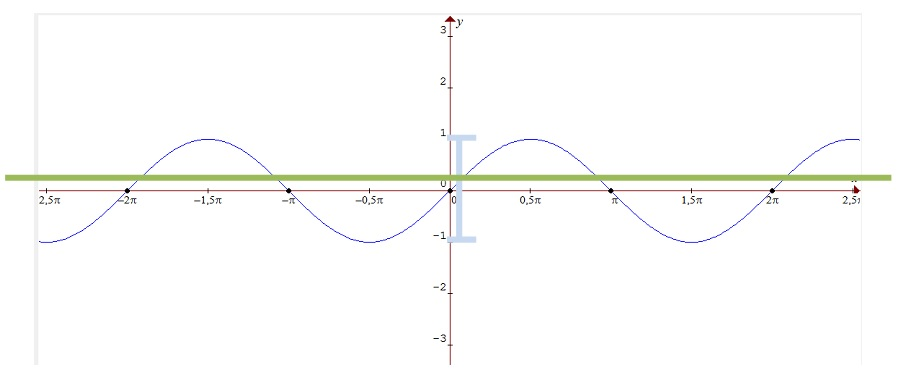
\includegraphics[height=5cm]{2_elem_rekenvaardigheden_B/inputs/reeel_vb3.jpg} 
%\end{figure}

%TODO figuur inladen
\begin{figure}
	\centering          
	
\begin{center}
\begin{tikzpicture}[scale=1,cap=round]

% Styles
\tikzstyle{axes}=[]
\tikzstyle help lines=[color=blue!50,very thin,dotted]


%%%%%%%%%%%%%%%%%%%%%%%%%%%%%%%%
%		GRID
%%%%%%%%%%%%%%%%%%%%%%%%%%%%%%%%

\draw[style=help lines,step=1cm] (-3.9,-5.9) grid (3.9,5.9);



%%%%%%%%%%%%%%%%%%%%%%%%%%%%%%%%
%		ASSENSTELSEL
%%%%%%%%%%%%%%%%%%%%%%%%%%%%%%%%

\draw[->] (-5,0) -- (7,0) node[right] {$x$};
\draw[->] (0,-7) -- (0,7) node[left]{$y$};

%\draw[fill,cyan](1,1)circle [radius=0.025];

%\draw[red,cap=rect, loosely dashed, ultra thick, domain=-2:2] plot (\x, {(\x*\x-1)+0.05}) node[above,yshift=-.7cm, right]{};

%%%%%%%%%%%%%%%%%%%%%%%%%%%%%%%%
%legende
%%%%%%%%%%%%%%%%%%%%%%%%%%%%%%%%
%\tkzDefPoint(0.5,3.5){A}
%\tkzDefPoint(1,3.5){B}
%\tkzLabelPoint[right,xshift=+0.1cm](B){${\color{cyan}f(x)=|x^2-1|}$}
%\tkzDrawSegment[cyan,ultra thick](A,B)

%\tkzDefPoint(0.5,3.2){C}
%\tkzDefPoint(1,3.2){D}
%\tkzLabelPoint[right,xshift=+0.1cm](D){${\color{red}e(x)=x^2-1}$}
%\tkzDrawSegment[red,cap=rect, loosely dashed, ultra thick](C,D)


%%%%%%%%%%%%%%%%%%%%%%%%%%%%%%%%
%getallen op de x-as en lijntjes
%%%%%%%%%%%%%%%%%%%%%%%%%%%%%%%%   
\foreach \x/\xtext in {-4,-3,-2,-1,1,2,3,4}
	\draw[xshift=\x cm] (0pt,1pt) -- (0pt,0pt) node[below,fill=white]
	{$\xtext$};,3
	
%getallen op de y-as en lijntjes  
%BEGIN LUS
\foreach \y/\ytext in {-6,-5,-4,-3,-2,-1,1,2,3,4,5,6}
	\draw[yshift=\y cm] (1pt,0pt) -- (0pt,0pt) node[left,fill=white]
	{$\ytext$}; %EINDE LUS



%%%%%%%%%%%%%%%%%%%%%%%%%%%%%%%%
%		GRAFIEKEN
%%%%%%%%%%%%%%%%%%%%%%%%%%%%%%%%
%\draw[cyan,cap=rect,thick, domain=-6:6] plot (\x, \x) node[above, right]{${\color{cyan}y=x}$};

\draw[cyan,cap=rect,ultra thick, domain=-1.2:3.5] plot (\x, {
	pow(\x,3)-3*pow(\x,2)		% <- plaats het functievoorschrift hier
}) node[above]{$f(x)=x^3-3x^2$};

 
%node[blue]{stijgen} 
%\draw[cyan,cap=rect,ultra thick, domain=2.25:6] plot (\x, {(\x-2)^(-1)}) node[above,yshift=+0.5cm,left]{$\color{cyan} y=\frac{1}{x-2}$};


%\draw[cyan,cap=rect,ultra thick, domain=-7:1.9] plot (\x, {exp{\x}}) node[above, right]{${\color{cyan}y=\exp{x}}$};

%%%%%%%%%%%%%%%%%%%%%%%%%%%%%%%%
%		MARKERINGEN
%%%%%%%%%%%%%%%%%%%%%%%%%%%%%%%%
%verticale lijn
%\draw[-o,line width=4,teal, cap=rect,opacity=0.3] (0,-4) -- (0,0.25) node[right] {};
%\draw[line width=4,teal, cap=rect,opacity=0.3] (0,0) -- (0,4.2) node[right] {bld $f$ = $\mathbb{R}_0$};
%horizontale lijn

 \draw[white,fill=blue,opacity=.5] (1,-2) circle [radius=.1]   node[blue, above,xshift=-1.1cm,opacity=1] {buigpunt in $(1,-2)$};


 
\draw[teal,cap=rect,line width=4, opacity=.5, domain=.5:1.5] plot (\x, {
	-2-3*(\x-1)		% <- plaats het functievoorschrift hier
}) node[opacity=1,above]{};


\draw[] (1.5,1.5) node[blue] {hol of concaaf};
\draw[] (1.5,-5) node[blue] {bol of convex};

\end{tikzpicture}
\end{center}

	\caption{voorbeeld 3}
	\label{fig:reele_functies_vb3}	
\end{figure}


\textbf{Domein}: we mogen op de plaats van $x$ gelijk welke
hoek invullen, de sinus zal steeds bestaan.

Besluit: $\textrm{dom}\:y=\mathbb{R}$ 




\textbf{Beeld}: we lezen op de $y$-as het beeld af. De
functiewaarden voor de sinus kunnen nooit groter zijn dan $1$ of
kleiner dan $-1$

Besluit: $\textrm{bld}f=[-1,1]$




\textbf{Nulpunten}: de $x$-as wordt gesneden als $\sin(x)=0$.
Dit gebeurt zowel voor $x$-waarden gelijk aan $\{0,\pi,2\pi,3\pi,...\}$
als ook voor $\{...,-3\pi,-2\pi,-\pi,0\}$

Besluit: de snijpunten met de $x$-as zijn de punten $\{...,(-2\pi,0),(-\pi,0),(0,0),(\pi,0),(2\pi,0),...\}$
of iets korter genoteerd als: $\{(k\pi,0)\:\textrm{met}\:k\in\mathbb{Z}\}$




\textbf{Symmetrie}: via de goniometrische formules vinden
we snel dat $f(-x)=\sin(-x)=-\sin(x)=-f(x)$ , dus kunnen we zeggen
dat deze functie oneven is (symmetrisch t.o.v. de oorsprong).

\end{voorbeeld}